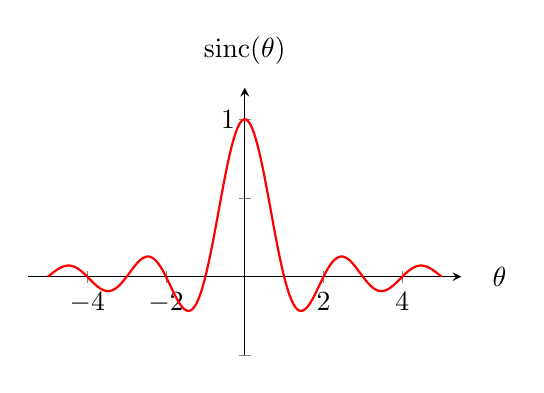
\begin{tikzpicture}
\begin{scope}	
    \begin{axis}[
		y=2cm,
		x=0.5cm,
		 clip=false,
		 xmin=-5.5,xmax=5.5,
		 xlabel= $\theta$,
		 ylabel={$\mathrm{sinc}(\theta)$},
		 ymin=-0.5,ymax=1.2,
		 axis lines=middle,
         	%xtick={-5, -4, ..., 5},
		 %ytick={-1, 1},
		 yticklabels=\empty,
		 every axis x label/.style={at={(ticklabel* cs:1.05)}, anchor=west,},
		every axis y label/.style={at={(ticklabel* cs:1.05)}, anchor=south,},
     ]
		%\addplot+[red, smooth, mark=none] table [x={n}, y={xn}] {periodic_square_fs_samples_of_envilope_gen.dat};
		\addplot [red, thick, domain=-5:5, samples=200] plot{sin(pi*deg(x))/(pi*x)};
		\node at (axis cs:0, 1) [anchor=east] { $1$ };
    \end{axis}
\end{scope}
\end{tikzpicture} 